%%%%%%%%%%%%%%%%%%%%%%%%%%%%%%%%%%%%%%%%%%%%%%%%%%%%%%%%%%%%%%%%%%%%%%%%%
%
%
%
%%%%%%%%%%%%%%%%%%%%%%%%%%%%%%%%%%%%%%%%%%%%%%%%%%%%%%%%%%%%%%%%%%%%%%%%%
\section{The nuclear fuel cycle}
The nuclear fuel cycle encompasses the activities and processes 
for the use of fissile materials in fission nuclear reactors 
\cite{tsoulfanidis_nuclear_2013}. 
Uranium, thorium, or plutonium can be used as 
fuel for a reactor, with this work, and most reactor designs, focusing on 
a uranium-based 
fuel cycle. The nuclear fuel cycle begins with the mining of uranium ores 
from the earth and ends with the final disposal of the radioactive 
waste produced 
\cite{tsoulfanidis_nuclear_2013}. A fuel cycle can vary based on the
design of the reactor(s) deployed, such as if enrichment is required.  
Figure \ref{fig:fuel_cycle} shows 
an example of the major steps in a nuclear fuel cycle. 

\begin{figure}
    \centering
    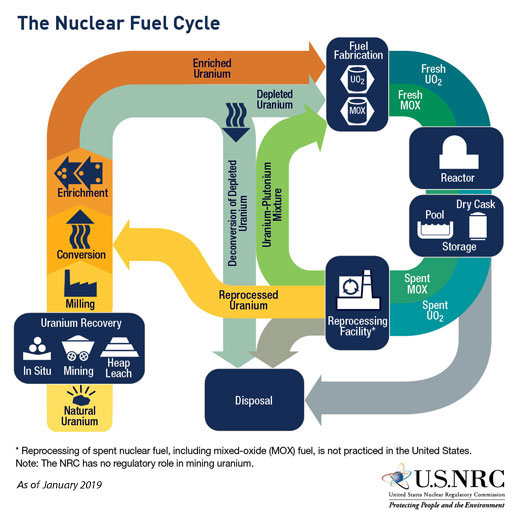
\includegraphics[scale=0.7]{nuclear_fuel_cycle.jpg}
    \caption{A complete view of options available for a once-through and 
    a recycling nuclear fuel cycle. Reproduced from 
    \protect\cite{us_nuclear_regulatory_commission_stages_2020}.}
    \label{fig:fuel_cycle}
\end{figure}

The \gls{NFC} has two primary sections: the front-end and 
the back-end. 
The front end encompasses the steps before the fuel arrives at a reactor 
and the back-end encompasses the steps after the fuel is discharged 
from the reactor \cite{rodriguez-penalonga_review_2017}. The front-end of 
the \gls{NFC} is often independent of the back-end, but the back-end 
of the \gls{NFC} is highly dependent on the front-end and the reactor 
type because they govern the form and composition of the discharged 
\gls{SNF}. The front-end of the fuel cycle includes the mining, 
milling, conversion, and enrichment of uranium, as well as 
fuel fabrication. The mining step is the physical extraction of uranium 
ore from the earth's crust. Milling removes the non-uranium containing 
parts of the ore to purify the ore into yellow-cake uranium (U$_3$O$_8$).
The conversion step changes the chemical state of uranium compound 
for the next step in the fuel cycle. If enrichment is present, conversion 
changes the yellow-cake uranium to UF$_6$. If enrichment is not 
needed, then the uranium is converted to whatever chemical compound is 
needed for the fuel fabrication process. Enrichment modifies the 
relative abundance of different isotopes in the uranium, specifically 
to increase the abundance of $^{235}$U compared with $^{238}$U. Fuel 
fabrication then converts the (enriched) uranium to the chemical 
form required by the reactor(s) deployed. For \glspl{LWR}, fuel 
fabrication converts the enriched uranium into a UO$_2$ ceramic 
pellet. Other reactor designs may require that fuel fabrication 
produce a UCO \gls{TRISO} pebble, a molten salt, or a metallic fuel. 

The back-end of the fuel cycle can also vary, primarily based on if spent 
fuel is reprocessed before final disposal. This variation in the 
back-end of the fuel cycle results in different names for the fuel 
cycle, based on if reprocessing is included: a once-through and a recycling 
(or twice-through) fuel cycles \cite{tsoulfanidis_nuclear_2013}. 

\subsection{Once-through fuel cycle}
A once-through fuel cycle is characterized by \gls{SNF} disposal
after being discharged from a reactor, and not undergoing any chemical processes 
or treatments \cite{rodriguez-penalonga_review_2017}. The gray line from 
the storage to disposal in Figure \ref{fig:fuel_cycle} represents 
the back-end of a once-through fuel cycle. This fuel cycle does 
not include any of the material flows from the ``Reprocessing Facility'' 
in Figure \ref{fig:fuel_cycle}.
This is the fuel cycle option currently employed in the 
United States. 

Once-through \glspl{NFC} use interim and final disposal schemes
\cite{rodriguez-penalonga_review_2017}. One form of interim 
storage, used regardless of 
the fuel cycle option, is cooling in an \textit{in situ} pool. 
This interim storage step can last between 3-10 years after reactor 
discharge \cite{rodriguez-penalonga_review_2017}
and provides active cooling to the \gls{SNF}.
Another form of interim storage is dry cask storage, located 
on-site or at a centralized location, which provides passive 
cooling to the \gls{SNF} after active cooling in a pool. 
Final disposal, which takes the form of a 
deep geologic repository, is the ultimate disposal of \gls{SNF} and 
is needed in both a once-through and recycling fuel cycle. The 
US has currently identified Yucca Mountain as a geologic repository 
site, but it is currently not operating.  

\subsection{Recycling fuel cycle}
A recycling fuel cycle is characterized by \gls{SNF} undergoing chemical 
processes to separate out uranium, plutonium, and other 
actinides from the fuel for use in a reactor again \cite{rodriguez-penalonga_review_2017}. 
Reuse of \gls{SNF} is possible because it consists of 95-97\% uranium and 
plutonium \cite{rodriguez-penalonga_review_2017}, which can fission and 
produce energy in a nuclear reactor. A \gls{NFC} that includes 
recycling is often referred to as ``closed fuel cycle'', because material is 
put back into the fuel cycle and a diagram of material flow forms 
a complete circle, as shown by the arrows from the ``Reprocessing Facility''
node in Figure \ref{fig:fuel_cycle}. 
There are two types of recycling fuel cycle options: a limited 
recycle scheme and a continuous recycle scheme \cite{wigeland_nuclear_2014}. 
A limited recycling scheme involves fuel being reprocessed and burned in 
a reactor for a finite number of times before final disposal. A continuous 
recycle scheme involves fuel being repeatedly reprocessed and burned in 
a reactor. An 
important difference between these two schemes is that \gls{SNF} is 
disposed of in a limited recycle scheme, but not in the continuous 
recycle scheme. Therefore, the recycling scheme will affect the amount of 
new resources (uranium) that must be acquired and the amount of material 
sent for final disposal in a repository. 

There are two primary methods to reprocess \gls{SNF}: aqueous reprocessing 
and pyroprocessing. Aqueous reprocessing relies on redox reactions of 
select actinides (typically uranium and plutonium) to move the 
actinides from an aqueous phase to an organic phase, while the non-desired 
materials in the \gls{SNF} remain in the aqueous phase \cite{rodriguez-penalonga_review_2017}. 
There 
are a variety of methods to perform aqueous reprocessing, with each method 
removing different combinations of elements from the \gls{SNF}, but the primary 
method is the PUREX process. The separated uranium and plutonium from 
aqueous reprocessing are then fabricated into \gls{MOX} fuel for use in 
a thermal-spectrum reactor. \gls{MOX} fuel can go through a limited number 
passes in a thermal reactor before disposal \cite{rodriguez-penalonga_review_2017}.
Pyroprocessing uses electric potentials to 
pull actinides (uranium and 
\glspl{TRU}) onto a cathode from a molten salt bath, while the fission products
remain in the molten salt bath or on the anode. The 
separated U/\gls{TRU} material from pyroprocessing can then be fabricated 
into metallic fuel for use in a fast-spectrum reactor. 
The \gls{SNF} from 
the fast reactor can be reprocessed multiple times and continuously put back 
into a reactor. Although this technique 
has a smaller separation factor than aqueous reprocessing, fast-spectrum 
reactors are less sensitive to impurities in the fuel and can readily use 
fuel fabricated after pyroprocessing \cite{rodriguez-penalonga_review_2017}.
Aqueous reprocessing is commercially available, and used in 
France, but pyroprocessing is not commercially available 
\cite{rodriguez-penalonga_review_2017,noauthor_status_2021}. 

Reprocessing \gls{SNF} improves resource utilization, compared 
with a once-through fuel cycle. One estimate reports that uranium ore
requirements would decrease by 25\% annually if \gls{SNF} is reprocessed 
to create \gls{MOX} fuel for \glspl{LWR} \cite{widder_benefits_2010}. 
Although this decrease in uranium ore requirements may improve the 
sustainability of the nuclear fuel cycle, current estimates of uranium 
reserves are expected to last for another 50-100 years 
\cite{widder_benefits_2010}. Therefore, reducing natural uranium usage  
is only of concern 
if there is an increase in the price of uranium ore. Another known benefit 
of reprocessing is the reduction in the volume and radioactivity of 
waste sent to a final repository. Reprocessing can reduce the waste 
volume by 
a factor of four by reprocessing \gls{SNF} \cite{widder_benefits_2010}, 
reducing the capacity of a repository required to store all the 
waste.
The radioactivity of the disposed waste decreases to about 10\% of the 
initial amount \cite{rodriguez-penalonga_review_2017} when employing 
recycling. Recycling \gls{SNF} reduces the concentration of actinides 
that are disposed of, which are the primary contributor to the long-term 
radioactivity of waste. 

Despite these benefits, recycling has known disadvantages compared to 
a once-through fuel cycle.
The amount of \gls{LLW} generated greatly increases by using 
reprocessing \cite{widder_benefits_2010}. The \gls{LLW} generated 
from reprocessing includes any solvents or materials used for the process 
and must be disposed of in accordance with regulations, but not 
necessarily in a deep geologic repository.
Pyroprocessing reduces the amount of \gls{LLW} compared with 
a once-through fuel cycle more than aqueous reprocessing because
the molten salt bath used in pyroprocessing can be cleaned 
and re-used. The \gls{LLW} generated demonstrates how the reprocessing 
technology employed affects the performance of the fuel cycle. 
Additionally, reprocessing has an increased 
proliferation risk. Aqueous reprocessing creates a material stream of 
pure plutonium \cite{widder_benefits_2010}, which can be diverted to 
create a nuclear weapon. This concern led to the development of new 
methods to reprocess \gls{SNF} without creating pure plutonium, such 
as the NUEX and COEX reprocessing methods \cite{widder_benefits_2010}. 
Pyroprocessing has a reduced proliferation risk compared with 
aqueous reprocessing
because a plutonium material stream is never created. The extracted 
plutonium is always mixed with uranium and other \gls{TRU} material 
\cite{noauthor_status_2021}.
Additionally, reprocessing \gls{SNF} is expected to cost more than 
using a once-through fuel cycle \cite{rodriguez-penalonga_review_2017,widder_benefits_2010}. 
The estimated 
\gls{LCOE} are \$30-75/MWh for a once-through fuel cycle, with an 
average of about \$47/MWh, and \$35-81/MWh for a fuel 
cycle with reprocessing, with an average of about \$52/MWh 
\cite{widder_benefits_2010}. The ranges in the \gls{LCOE} come from 
differences in assumptions in determining the costs. Based on these 
estimates, there is no economic incentive to reprocess and recycle 
\gls{SNF}, unless the cost of mining fresh uranium were to increase. 

As discussed with the amount of waste produced, each reprocessing method 
has their own advantages and disadvantages. 
A comparison of fuel cycle options for the Republic of Korea 
showed that using pyroprocessing with \glspl{SFR} required less natural 
uranium than both a once-through fuel cycle and using aqueous reprocessing 
and fewer \glspl{PWR} to produce the same amount of energy 
\cite{park_comparative_2011}. Both methods of reprocessing  
reduced the amount of \gls{SNF} for disposal,
but using pyroprocessing with a fast reactor produced no \gls{SNF} for 
disposal. This occurred because the separated material from 
pyroprocessing that cannot be recycled in a reactor is assumed to be 
disposed of as \gls{LLW} in the analysis. One disadvantage of reprocessing 
identified by Park et al. is the increase in \gls{LLW} produced 
when using aqueous reprocessing and 
thermal reactors. This result is consistent with the analysis 
by \cite{widder_benefits_2010}, which showed a decrease in \gls{LLW} 
mass when using a fuel cycle with pyroprocessing and fast reactors, 
compared with a once-through fuel cycle \cite{park_comparative_2011}. 

\section{Uranium enrichment}
In the \gls{NFC}, enrichment increases the relative abundance of 
$^{235}$U compared with $^{238}$U in the fuel, increasing
the relative abundance of fissile material needed 
for most reactor designs. There are multiple technologies and processes that can 
enrich uranium, including gaseous diffusion, calutrons, and laser separation 
technologies. The US currently employs gaseous centrifuges to enrich uranium 
for commercial supplies. Gaseous centrifuges are currently 
used at the Urenco site in New Mexico \cite{us_nuclear_regulatory_commission_louisiana_2022} and 
planned for the Centrus facility in Piketon, Ohio 
\cite{us_nuclear_regulatory_commission_centrus_2021}. Gaseous centrifuges 
are rotating canisters, 
relying on the speed of the rotation to move heavier 
materials to the outside of the canister. Because of this preferential 
movement, a greater concentration of the lighter material ($^{235}$U) 
accumulates near the middle of the canister \cite{villani_uranium_1979}. 
To ensure that only the mass difference in the uranium isotopes causes 
this preferential separation, the uranium is sequestered in UF$_6$ gas, because 
fluorine only has one naturally occurring isotope. Therefore, the 
fluorine present does not contribute to any mass differences between 
different molecules. 

Multiple quantities govern the capacity of an enrichment facility 
\cite{tsoulfanidis_nuclear_2013}, defined in Table \ref{tab:enrichment_variables}.
Each of these quantities can be related using the following equations:
\begin{subequations}
    \begin{equation}
        F = P + T
    \end{equation}
    \begin{equation}
        x_fF = x_pP + x_tT
        \label{eq:enrichment_assasys}
    \end{equation}
    \begin{equation}
        SWU = \left[P*V(x_p) +T*V(x_t) - F*V(x_f)\right]*t
        \label{eq:swu}
    \end{equation}
    \text{in which:}
    \begin{equation}
        V(x_i) = (2x_i - 1)*\ln\left(\frac{x_i}{1-x_i}\right)
        \label{eq:sep_potential}
    \end{equation}
    \label{eq:enrichment}
\end{subequations}

\begin{table}
    \centering
    \caption{Definitions for variables used to describe throughput and 
    capacity for an enrichment facility.}
    \label{tab:enrichment_variables}
    \begin{tabular}{c c c}
        \hline
        Variable & Description & Units\\\hline
        F & Mass of feed material per unit time & kg\\
        P & Mass of product material per unit time & kg \\
        T & Mass of tails material per unit time & kg\\
        x$_f$ & weight fraction of $^{235}$U in the feed stream &\\
        x$_p$ & weight fraction of $^{235}$U in the product stream & \\
        x$_t$ & weight fraction of $^{235}$U in the tails stream & \\
        \gls{SWU} & the physical work required to separate the isotopes & kg-SWU\\
        t & time step & d\\
        \hline
    \end{tabular}
\end{table}

\noindent The \acrfull{SWU} capacity 
is the physical work required to put into the system to provide the 
separation needed to meet the product stream demand. It is also related 
to the amount of energy the facility 
requires \cite{tsoulfanidis_nuclear_2013}. 

The equations in Eq. \ref{eq:enrichment} show that as the desired enrichment level 
of the product feed increases, the feed mass must also increase, assuming everything 
else is held constant. The equations also show that as the desired 
product 
enrichment level increases, the amount of \gls{SWU} capacity needed also increases. 
However, if the product mass decreases, then the required \gls{SWU} capacity 
also decreases. Therefore, changes to the product enrichment level and mass 
throughput have similar effects on the amount of feed material and required 
\gls{SWU} capacity. Opposing changes to both quantities 
(i.e., an increase in one and a decrease in the other) will not lead to a clear 
expectation for the change in feed material of the \gls{SWU} capacity. 
The effect on these variables will depend on the magnitude of the changes.

The separation needed to enrich uranium cannot be performed 
in a single 
separation step because of the separation efficiency of gas centrifuges. 
Therefore, centrifuges at a facility have  
cascades, as shown in Figure \ref{fig:cascade}. Each cascade is designed with 
multiple separation stages in series, with multiple centrifuge units in 
parallel comprising each stage \cite{villani_uranium_1979}. Each stage 
outputs a product enriched to a certain amount (less than the final product 
of the cascade), then the product from one 
stage becomes the feed material for the next stage in the cascade to produce 
a greater enrichment level. The tails material from each 
stage is combined with feed material for the previous stage, to help strip 
out any $^{235}$U that is left in the tails. Using the tails in the 
previous stage develops the cascade into a counter-current cascade 
\cite{villani_uranium_1979} and helps to improve the efficiency of the entire cascade. 
Changing the product stream assay (the $^{235}$U weight fraction)
requires a change in the cascade configuration of 
a facility, even if the required \gls{SWU} capacity is the same. Therefore, 
understanding the product stream assay, \gls{SWU} capacity needed, and the 
amount of product needed aids in designing facilities to meet potential 
demand of \gls{HALEU}.

\begin{figure}
    \centering
    \begin{tikzpicture}[node distance=1.5cm]
        \node (C1) [centrifuge] {};
        \node (C2) [centrifuge, below of=C1] {};
        \node (C3) [centrifuge, below of=C2] {};
        \node (C4) [centrifuge, below of=C3] {};
        \node (C5) [centrifuge, below of=C4] {};
        \node (C6) [centrifuge, below of=C5] {};
        \node (C7) [centrifuge, right of=C1, xshift=2.5cm, yshift=-0.75cm] {};
        \node (C8) [centrifuge, below of=C7] {};
        \node (C9) [centrifuge, below of=C8] {};
        \node (C10) [centrifuge, below of=C9] {};
        \node (C11) [centrifuge, below of=C10] {};
        \node (C12) [centrifuge, right of=C7, xshift=2.5cm, yshift=-0.75cm] {};
        \node (C13) [centrifuge, below of=C12] {};
        \node (C14) [centrifuge, below of=C13] {};
        \node (C15) [centrifuge, below of=C14] {};
        \node (label1) [draw=none, fill=none, above of=C7, yshift=2cm] {Cascade};
        \node (label2) [draw=none, fill=none, below of=label1] {Stage};

        
        \draw [arrow] (-3,-3.75)--(-2,-3.75);
        \draw (-2,0) -- (-2,-7.5);
        \draw [arrow] (-2,0) -- (-1,0);
        \draw [arrow] (-2,-1.5) -- (-1,-1.5);
        \draw [arrow] (-2,-3) -- (-1,-3);
        \draw [arrow] (-2,-4.5) -- (-1,-4.5);
        \draw [arrow] (-2,-6) -- (-1,-6);
        \draw [arrow] (-2,-7.5) -- (-1,-7.5);
        \draw [arrow] (1,0) -- (1.75,0);
        \draw [arrow] (1,-1.5) -- (1.75,-1.5);
        \draw [arrow] (1,-3) -- (1.75,-3);
        \draw [arrow] (1,-4.5) -- (1.75,-4.5);
        \draw [arrow] (1,-6) -- (1.75,-6);
        \draw [arrow] (1,-7.5) -- (1.75,-7.5);
        \draw (1.75,0) -- (1.75,-7.5);
        \draw [arrow] (1.75,-3.75)--(2.25,-3.75);
        \draw (2.25,-0.75) -- (2.25,-6.75);
        \draw [arrow] (2.25,-0.75) -- (3,-0.75);
        \draw [arrow] (2.25,-2.25) -- (3,-2.25);
        \draw [arrow] (2.25,-3.75) -- (3,-3.75);
        \draw [arrow] (2.25,-5.25) -- (3,-5.25);
        \draw [arrow] (2.25,-6.75) -- (3,-6.75);
        \draw [arrow] (5,-0.75) -- (5.75,-0.75);
        \draw [arrow] (5,-2.25) -- (5.75,-2.25);
        \draw [arrow] (5,-3.75) -- (5.75,-3.75);
        \draw [arrow] (5,-5.25) -- (5.75,-5.25);
        \draw [arrow] (5,-6.75) -- (5.75,-6.75);
        \draw (5.75,-0.75) -- (5.75,-6.75);
        \draw [arrow] (5.75,-3.75)--(6.25,-3.75);
        \draw (6.25,-1.5) -- (6.25,-6);
        \draw [arrow] (6.25,-1.5) -- (7,-1.5);
        \draw [arrow] (6.25,-3) -- (7,-3);
        \draw [arrow] (6.25,-4.5) -- (7,-4.5);
        \draw [arrow] (6.25,-6) -- (7,-6);
        \draw [arrow] (6.25,-1.5) -- (7,-1.5);
        \draw [arrow] (6.25,-3) -- (7,-3);
        \draw [arrow] (6.25,-4.5) -- (7,-4.5);
        \draw [arrow] (6.25,-6) -- (7,-6);
        \draw (9.75,-1.5) -- (9.75,-6);
        \draw [arrow] (9, -1.5) -- (9.75,-1.5);
        \draw [arrow] (9, -3) -- (9.75,-3);
        \draw [arrow] (9, -4.5) -- (9.75,-4.5);
        \draw [arrow] (9, -6) -- (9.75,-6);
        \draw [arrow] (9.75,-3.75)--(10.5,-3.75);

        \draw [dashed] (-2,0) -- (-2,3);
        \draw [arrow] (label1) -- (-2,2.75);
        \draw [dashed] (9.75,-3) -- (9.75,3);
        \draw [arrow] (label1) -- (9.75,2.75);
        \draw [dashed] (2.25,-1.5) -- (2.25,1.5);
        \draw [arrow] (label2) -- (2.25, 1.25);
        \draw [dashed] (5.75,-1.5) -- (5.75,1.5);
        \draw [arrow] (label2) -- (5.75, 1.25);
        \end{tikzpicture}
    \caption{Diagram of material flow through an enrichment facility 
    cascade. The lines and arrows shown are the product stream from each unit, and the 
    tails stream is not shown. Each box represents a single centrifuge, or 
    unit. How the units comprise a stage, each vertical column,
    and the cascade, the entire configuration, are identified. 
    Figure recreated from \protect\cite{villani_uranium_1979}.}
    \label{fig:cascade}
\end{figure}

The design parameters for a cascade are optimized based on the separation 
factor 
achieved in the centrifuges, the flow rate, and the material assays. 
The required product assay and the separation factor of each stage govern 
the number of stages required in a cascade \cite{whitaker_uranium_2019}. 
Therefore, to achieve a higher product assay either more stages 
need to be added or each stage needs to achieve a greater separation
factor. The product flow rate governs the number of centrifuges in 
each stage \cite{whitaker_uranium_2019}. As the flow rate increases, 
so do the number of centrifuges per stage. 


%%%%%%%%%%%%%%%%%%%%%%%%%%%%%%%%%%%%%%%%%%%%%%%%%%%%%%%%%%%%%%%%%%%
%
%
%
%%%%%%%%%%%%%%%%%%%%%%%%%%%%%%%%%%%%%%%%%%%%%%%%%%%%%%%%%%%%%%%%%%%
\section{Fuel cycle simulators}
\gls{NFC} simulators are computational tools to model the flow of materials
and the commissioning and decommissioning of facilities for a given fuel 
cycle. \gls{NFC} simulators can evaluate the transition between fuel cycle 
options (e.g., from a once-through to a recycling fuel cycle), the 
performance of one fuel cycle with a growth in the demand of nuclear power, 
and the effect of perturbations on a given fuel cycle \cite{piet_dynamic_2011}. 

\gls{NFC} simulators can include multiple functionalities, 
such as material flow tracking and facility deployment \cite{brown_identification_2016}.
Foundational capabilities of an \gls{NFC} simulator include modeling 
facility deployment and retirement, fuel materials, timing and capacity of 
facilities, and external sources of fissile material (such as a mine) 
\cite{brown_identification_2016}. Each of these features can then be 
expanded upon through `integral' or `exemplary' features to expand the 
foundational capabilities. Examples of `integral' 
features include strategic deployment of facilities to meet a specified 
material demand or material prioritization. Examples of `exemplary' 
features include modeling radioactive decay of materials or calculations 
of fuel depletion in a reactor \cite{brown_identification_2016}. 

A variety of fuel cycle simulators have been developed, often to focus on 
specific areas of the nuclear fuel cycle \cite{huff_next_2010}. Some of the 
\gls{NFC} simulators developed include
\gls{DYMOND} \cite{feng_sensitivity_2020,feng_standardized_2016}, 
\gls{VISION} \cite{yacout_visionverifiable_2006}, and ORION 
\cite{gregg_analysis_2012}.
\gls{DYMOND} is a fuel cycle simulator developed by \gls{ANL} initially for 
the Gen IV Fuel Cycle Crosscut Group. This simulator combines 
multiple modeling paradigms, including system dynamics, discrete events, and
agent-based modeling \cite{feng_standardized_2016,feng_sensitivity_2020}.
\gls{DYMOND} accepts inputs of reactor and fuel characteristics, fuel cycle 
facility properties, the facilities that use each fuel type, and an 
energy demand to output the reactor fleet composition \cite{feng_standardized_2016}.
One distinguishing 
feature of \gls{DYMOND} is that it performs depletion of material inputs 
to a reactor facility using ORIGEN, enabling 
an `exemplary' functionality of \gls{NFC} simulators. 
\gls{VISION} was developed primarily to meet the program objectives of the 
\gls{AFCI} and is based on \gls{DYMOND} \cite{yacout_visionverifiable_2006}.
\gls{VISION} was initially developed to be US-focused, but has been modified to 
be more generalized in its capabilities \cite{feng_standardized_2016}.
\gls{VISION} dynamically models the mass flow of material through the 
entire fuel cycle and calculates metrics based on the \gls{AFCI} program 
objectives. New functionalities added to \gls{VISION}, compared with \gls{DYMOND}, 
include estimating economic costs and modeling isotope decay. 
\gls{VISION} has multiple 
modules to model the mass flow, calculate metrics, perform control, or 
integration. 
Both \gls{DYMOND} and \gls{VISION} model the fuel cycle at a fleet level, 
instead of a facility level \cite{feng_standardized_2016}.  
The UK National Nuclear Laboratory developed ORION, which tracks up to 
2500 nuclides as they 
move through a nuclear fuel cycle \cite{gregg_analysis_2012}. ORION models
facilities as individual objects, instead of just at the fleet level, and 
the decay and irradiation of the tracked nuclides 
\cite{feng_standardized_2016}.

Another \gls{NFC} simulator is \Cyclus, an open-source, agent-based 
\gls{NFC} simulator \cite{huff_fundamental_2016}. The next section 
describes \Cyclus more in-depth as it is the simulator chosen for this 
work. 

\subsection{\Cyclus}
\Cyclus is a dynamic, open source agent-based fuel cycle simulator. Built 
in C++, \Cyclus uses only open source and freely available libraries to 
provide full access to all users and developers. The 
\Cyclus architecture treats materials and facilities independently, similar 
to ORION, and allows 
for variable fidelity levels \cite{huff_fundamental_2016}. These attributes
of \Cyclus allow for the software to easily model any fuel cycle scenario.

\Cyclus uses the notion of an \textit{agent} to represent different 
components in the simulated fuel cycle. Agents are 
defined using the \Cyclus \gls{API}, which allow 
users 
to develop their own suite of agent libraries and use them within \Cyclus. 
The \gls{API} anticipates the structure on information about a given 
library 
required by the core \Cyclus kernel, facilitating 
information sharing between the plug-in library and the \Cyclus framework. 
In addition to the flexibility in libraries and agents, this framework 
also allows for flexibility in licensing and distribution of the user 
defined libraries. Libraries are loaded without changes to the \Cyclus 
kernel and without unwanted transfer of sensitive information. This lack 
of information transfer allows library development with export controlled 
software but still allow \Cyclus to be open-source.

The agent-based modeling paradigm employed by \Cyclus allows agent level 
modeling, as opposed to system level modeling. This paradigm allows different 
fuel cycle facilities, such as a reactor and a fuel fabrication plant, to 
be defined independently but still interact with each other in the 
simulation. There are three main groups of agents within the \Cyclus 
architecture: facilities, institutions, and regions. Facilities are 
the individual units in the fuel cycle that implement technology, 
such as a fuel fabrication facility or a uranium mine. Institutions 
manage the facilities, similar to how a company manages facilities. 
Regions provide geographic 
and political context for the institutions and regions and can be thought 
of as similar to individual nations. The types of agents are related using 
a parent-child hierarchy: regions are
parents of institutions, and institutions are parents of facilities. This 
structure places the responsibility of deploying and decommissioning 
facilities with the institutions. 

The \Cycamore agent library provides a variety of libraries that can be 
dynamically loaded into \Cyclus for use in a simulation 
\cite{huff_fundamental_2016,carlsen_cycamore_2014}. These libraries 
include multiple facilities, two institutions, and one region as of 
\Cycamore 1.3 \cite{huff_fundamental_2016}. The two institutions interact 
with the region (the \Cycamore \texttt{GrowthRegion}) to deploy 
facilities as needed to meet a commodity demand specified by the region. 
The \Cycamore \texttt{DeployInst} manually defines the number of each 
facility to be deployed at each time step. These facilities 
registered with the \Cycamore \texttt{GrowthRegion} for their 
contribution to the demand and are decommissioned at the end of their 
lifetime. The 
\Cycamore \texttt{ManagerInst} calculates the number of each facility 
type to deploy to meet the demand given by the \texttt{GrowthRegion}, 
based on what is not met through facilities deployed by other institutions 
in the region.  

In \Cyclus, agents trade materials through the \gls{DRE} 
\cite{gidden_agent-based_2015,huff_fundamental_2016}. The \gls{DRE} defines the 
supply-demand communication framework and treats facilities as black boxes
so the solution strategy is agnostic to the resource types being exchanged. 
The \gls{DRE} is a novel concept and unique to \Cyclus. It provides a 
flexible architecture to support supply-demand modeling and dynamic 
material flows between facilities \cite{huff_fundamental_2016}. 
There are three steps in the \gls{DRE}: information gathering, resource 
exchanges, and trade execution \cite{gidden_agent-based_2015}. 
During the information gathering 
phase facilities that need materials state their demand for a given 
material (e.g., a reactor stating a demand for fuel), referred to 
as requests. Requests 
from a facility can be more than what is actually required (e.g. a reactor
requesting extra fuel assemblies just in case one breaks mid-cycle). Additionally, 
facilities can state mutual requests, or state requests for materials in 
which either of the materials would meet the demand (e.g., a reactor 
requesting UOX and MOX fuel but only needing one to meet their request), with 
a preference defined for each material. Requests for materials can have 
constraints attached, such as quantity limits or if the request is 
\textit{exclusive}. Exclusive requests mean that it must be met fully 
from a single bid, as opposed to being met through multiple small 
bids. Then facilities that produce materials also state the amount of a 
material they have to trade away (e.g., a fuel fabrication plant stating 
that they have 3 fuel assemblies), as the responses to the requests or 
bids. Using the information of the material requests and the bids, 
an exchange graph is created. The exchange graph is a 
bipartite network \cite{gidden_agent-based_2015}
with nodes for the requests and the responses to the requests. 

Once the exchange graph is created, the requesting facilities can apply 
preferences to possible each potential bid based on the facility 
making the bid \cite{huff_fundamental_2016}. Preferences can be based on 
the facility making the bid, or the bidding facility's institution or 
region. For example, a reactor facility can prefer to receive fuel 
assemblies from one agent, or agents from an institution (mimicking but not 
fully enforcing contracts between companies), or agents from a region 
(mimicking international trade agreements). The addition of preferences of 
potential bids allows the \gls{DRE} to more closely mimic supply chain 
dynamics within a fuel cycle. 
A solution is found to the exchange graph by matching requests with 
responses. A feature of \Cyclus is that it is possible for 
requests to be unmet if there is not enough material in the responses 
to fully meet the bid. To account for this 
capability, unconstrained false nodes are defined in the exchange graph
to ensure a feasible solution is possible \cite{gidden_methodology_2016}.
A solution to the exchange graph is found using a simulation-based 
heuristic or a mathematical program \cite{gidden_agent-based_2015}.
Mathematical models to solve the exchange graph include \gls{MILP} and 
\gls{LP}, with \gls{MILP} required to solve the exchange graph if 
any of the requests are denoted as exclusive \cite{huff_fundamental_2016}.
Once a solution is found to the exchange graph, the materials are 
traded between the matched facilities in the trade execution phase.  

Similar to many of the other fuel cycle simulators developed, material 
compositions in \Cyclus are defined using recipes. Recipes are 
typically defined as stagnant compositions are the beginning of 
a simulation. However, there are instances in which fuel compositions 
need to be dynamic during a simulation, such as when accounting for fuel 
depletion. 

\subsection{Fuel depletion}
Fuel depletion is an important component of fuel cycle simulations 
because the composition of spent fuel affects the decay heat, 
amount of fissile material present, and the volume of the spent 
fuel. Each of these fuel properties affect transportation of the fuel, 
repository storage limits, and how much material is available for 
reprocessing and recycling. Therefore, fuel cycle simulators must 
have a way to account for fuel depletion. 

One possible way to account for fuel depletion is define stagnant 
compositions of spent fuel and update the fuel composition when 
it is discharged from a reactor. Spent fuel compositions are defined 
based on depletion modeling through other codes, and are applied 
to the modeled fuel cycle. This methodology is used by the 
\Cycamore Reactor archetype for \Cyclus \cite{carlsen_cycamore_2014}
and is available through ORION \cite{sunny_transition_2015}. The 
material compositions must be known \textit{a priori}, with spent fuel 
compositions typically obtained by modeling depletion before modeling the 
fuel cycle. 
This method of accounting for fuel depletion provides a fast and 
low-fidelity way to model a fuel cycle. Although it has been used to 
model closed fuel cycles \cite{bae_standardized_2019,djokic_application_2015},
it is most appropriate for once through fuel cycles 
\cite{sunny_transition_2015} because the same 
compositions for fresh fuel are loaded into a reactor at each 
refueling, which means that the spent fuel compositions do not vary 
greatly between discharged batches. 

Dynamic modeling of fuel depletion is considered an ``exemplary'' quality 
of a fuel cycle simulator by Brown et al. \cite{brown_identification_2016},
and is available in different simulators. ORION \cite{feng_standardized_2016}
and DYMOND \cite{richards_application_2021} both have dynamic fuel 
depletion capabilities that allow the codes to more accurately fuel depletion 
and the effects of fuel compositions on the fuel cycle. \gls{ORION} allows 
users to define material compositions through recipes or the code can 
model decay and depletion of material \cite{sunny_transition_2015}. ORION 
has some built-in reactor-specific cross sections for modeling 
depletion during a fuel cycle simulation, or users can generate 
and provide their own cross section data to fit the reactors and fuel cycle 
they are modeling. DYMOND models depletion through a coupling with 
ORIGEN2, a stand-alone depletion solver, using pre-generated 
reactor-specific depletion libraries \cite{richards_application_2021}.
The coupling of DYMOND with ORIGEN2 provides dynamic updates to 
spent fuel compositions, but it also allows for the code to perform 
criticality searches to determine fresh fuel compositions based on 
the spent fuel compositions available. This criticality search provides 
more accurate compositions of the fresh fuel produced than using a recipe 
to define the composition because it creates a feedback mechanism 
between the fresh and spent fuel compositions \cite{richards_application_2021}.
However, the increased accuracy in fuel compositions in DYMOND comes 
at the cost of increased computational cost \cite{richards_application_2021}.

The core kernel of \Cyclus does not provide a method to dynamically 
model depletion of fuel. However, the modular nature of \Cyclus means 
that developers can easily couple \Cyclus to a third-party code to 
model fuel depletion. One such coupling is \gls{CYBORG}, which is a 
reactor-style archetype that couples \Cyclus with ORIGEN 
\cite{skutnik_cyborg_2016}. \gls{CYBORG} leverages the validated 
depletion capabilities in ORIGEN to model fuel depletion during 
a fuel cycle simulation. \cite{skutnik_cyborg_2016}. Fresh fuel  
compositions and reactor parameters (such as irradiation time and 
power level) are passed from \Cyclus to \gls{CYBORG}, which then produces 
a problem-specific cross section library that is then passed to 
ORIGEN to perform the depletion calculation. The depleted material 
compositions are then passed back to \Cyclus to update the 
appropriate material compositions. Use of this 
archetype requires users to have a license to use ORIGEN, as it 
it an export-controlled code, which can pose issues in a user being 
able to use this archetype. Further development of depletion 
capabilities in \Cyclus include coupling it with other 
depletion solvers, such as OpenMC \cite{romano_depletion_2021}, 
or the development of an archetype with an internal CRAM solver. 
These additional capabilities could potential increase the user base 
for this capability because they would potentially not require a user 
to obtain a license to use the software. 

Another third-party archetype developed to account for fuel depletion 
is Bright-lite \cite{schneider_integrated_2016}. This archetype accounts for 
fuel depletion through two methods: forward calculations and blending. 
The forward method uses a defined input fuel composition to determine 
the spent fuel isotopics and fuel burnup using one-group cross 
section libraries. In the blending mode, the archetype uses two materials 
streams of known composition and combines them to reach a specified burnup 
for the fuel. Bright-lite creates a single cross section set for each 
fuel type and reactor condition. Each cross section set leads to a
isotope library database that contains the fluence, neutron production rate,
neutron destruction rate, total burnup, and isotope transmutation product 
vectors and matrices. 



\subsection{Verification and use of fuel cycle simulators}
Multi-lab efforts validated the \gls{NFC} simulators discussed here 
(\gls{DYMOND}, \gls{VISION}, ORION, and \Cyclus)
using a no growth transition from \glspl{LWR} 
to \glspl{SFR} \cite{feng_sensitivity_2020,bae_standardized_2019}.
Each \gls{LWR} in the scenario provides 1000 MWe of 
electricity and each \gls{SFR} provides 333.3 MWe of electricity. The 
scenario is simple enough that a spreadsheet could calculated the results, 
which served as an analytical solution. The 
results from each \gls{NFC} simulator were compared to each other and 
to the spreadsheet solution. Any observed differences were either explained 
based on modeling implementation or resolved through changes to the 
necessary code.

The results of the verification efforts showed agreement between each 
of the codes and the spreadsheet results, as well as identified modeling 
differences. For example, \gls{VISION} and \gls{DYMOND} model continuous 
reprocessing at each time step, as opposed to the instantaneous 
reprocessing modeled by the spreadsheet \cite{feng_standardized_2016}. 
This difference led to \gls{DYMOND} reporting lower annual mass flow 
rates for the \glspl{SFR} and a small delay in the idle \gls{SNF} 
inventory modeled by \gls{VISION} compared with the spreadsheet 
solution. 
Another difference identified is that the \Cycamore reactor 
archetype models each fuel assembly and batch as discrete material 
\cite{bae_standardized_2019}, as 
opposed to the other codes assuming continuous fuel discharge. 
This difference leads to oscillations in the \gls{SNF} discharged 
when using \Cyclus, while the other codes results do not have these 
oscillations.
However, this modeling decision in \Cyclus produced results that 
are closer to reality. 
Additionally, the \Cycamore reactor archetype depletes half of the 
core of fuel upon decommissioning, while the other \gls{NFC} simulators 
deplete the entire core of fuel upon decommissioning. This 
difference affects the \gls{TRU} material inventory, and was 
temporarily removed to demonstrate that the difference 
methodologies led to the difference in results \cite{bae_standardized_2019}.

A common use of \gls{NFC} simulators is to evaluate the performance 
of fuel cycles based on specific criteria. 
For example, work with \gls{DYMOND}, \gls{DANESS}, 
and \gls{NFCSim} evaluated how different fuel cycle options 
could reduce \gls{SNF} volume in a repository \cite{yacout_dynamic_2004}. 
\gls{NFC} simulators have also evaluated the transition between fuel cycle 
options. Dynamic simulations of fuel cycle options for the \gls{AFCI}
Campaign in 2005 demonstrate the importance of the magnitude, timing, 
and rate of deploying facilities for the new fuel cycle option 
\cite{piet_assessment_2011}.
Another common use of \gls{NFC} simulators is modeling the transition 
between 
different fuel cycle options or technology. Quantifying the transition 
between fuel cycle options occurs by studying metrics such as the 
energy output and resource requirements \cite{del_cul_advanced_2010}. 
Resource requirements can include the mass of natural uranium, enrichment 
needs, fuel irradiation, \gls{SNF}, waste production, and cost. 

The use of \gls{NFC} simulators over the 
last decade has primarily been guided by the Nuclear Fuel Cycle \gls{ES} 
from the \gls{DOE-NE} 
\cite{wigeland_nuclear_2014}. This project categorized 
multiple fuel cycle options into 40 different \glspl{EG} based on characteristics 
such as the recycling scheme, the type of fuel burned, 
and the type of reactor (e.g. thermal critical reactor, fast critical reactor). 
The \glspl{EG} were compared on their performance at equilibrium on nine evaluation 
criterion, including nuclear waste management and resource utilization. The 
results of this project showed that the most benefit comes from fuel cycles 
that use continuous recycling of U/Pu with new or natural uranium in fast critical 
reactors (\gls{EG} 23), continuous recycling of U/\gls{TRU} with new or natural 
uranium in fast critical reactors (\gls{EG} 24), continuous recycling of U/Pu 
with new or natural uranium in both fast and thermal critical reactors 
(\gls{EG} 29), or continuous recycling of U/\gls{TRU} with new or natural uranium in 
both fast and critical reactors (\gls{EG} 30) \cite{wigeland_nuclear_2014}. 

Based on the results of the \gls{ES}, many efforts have modeled 
the transition to these promising fuel cycle options using fuel cycle 
simulators. ORION modeled the transition from a once-through 
fuel cycle option using enriched uranium in thermal critical reactors 
(\gls{EG} 01 to \gls{EG} 29) \cite{sunny_transition_2015}. This work 
demonstrated the importance of new \glspl{LWR} and license 
extensions of existing reactors for this transition. 

\Cyclus has been used to model the transition from \gls{EG} 01 to \gls{EG} 
23 assuming a 1\% growth in power demand 
\cite{djokic_application_2015}. The results from \Cyclus were compared 
to the results from modeling the same transition scenario with \gls{DYMOND}. 
The power generated, reactor entry 
time, and reactor exit time for the \Cyclus simulation qualitatively 
matches well with the results of the \gls{DYMOND} simulation, but the power 
demand growth could match better to the target 1\% by slightly modifying 
the \gls{SFR} deployment. Littell \cite{littell_development_2016}
also modeled the \gls{EG} 01 to \gls{EG} 23 transition in \Cyclus. 
This work included constraints such as restricting the mass of separated 
plutonium to less than 100 MT, not allowing reprocessing to begin until 
at least 2050, and allowing up to 5\% surplus or deficit in the energy 
from compared with the demand. The capacity, deployment, and 
decommissioning of the reprocessing facilities must be tightly controlled
to achieve the stored plutonium limit. This control was needed 
because \Cyclus does not accept time-dependent facility storage capacities, 
and when there is no reprocessing facility capacity the stored plutonium 
limit was exceeded \cite{littell_development_2016}. 

%%%%%%%%%%%%%%%%%%%%%%%%%%%%%%%%%%%%%%%%%%%%%%%%%%%%%%%%%%%%%%%%%%%%%%%
%
%
%
%%%%%%%%%%%%%%%%%%%%%%%%%%%%%%%%%%%%%%%%%%%%%%%%%%%%%%%%%%%%%%%%%%%%%%%
\section{Sensitivity analysis and optimization}
Sensitivity analysis provides information on how each input parameter 
of a fuel cycle model affects output metrics. 
Performing this analysis identifies and quantifies the effect of input 
parameters on model outputs \cite{thiolliere_methodology_2018}. Sensitivity 
analysis is also useful because of the multiple sources of uncertainty in 
modeling the nuclear fuel cycle, such as facility design parameters, 
scenario assumptions, and reactor physics calculations 
\cite{noauthor_effects_2017}.
Sensitivity 
analysis simulates a fuel cycle multiple times 
with small perturbations in model inputs between each simulation. Then 
we observe the output metrics for any changes caused by each  
perturbation. Output metrics are presented through three different 
indicators: the final value, the maximum value, or the cumulative sum 
\cite{noauthor_effects_2017}. Thiolliere et al. 
\cite{thiolliere_methodology_2018} demonstrated a methodology to 
perform sensitivity analysis, defining the specific input parameters to 
perturb and the range of values those parameters can take.
They defined the range of values based on known technical capabilities, then 
sampled uniformly across the range of values to build the simulations. 
Feng et al. \cite{feng_sensitivity_2020} performed a similar methodology, 
using random sampling in the identified range of input variable values.
Some common
parameters varied during sensitivity analysis include the fuel burnup 
\cite{thiolliere_methodology_2018,noauthor_effects_2017}, the \gls{LWR}
lifetime \cite{feng_sensitivity_2020,noauthor_effects_2017}, 
and the transition start time or introduction date of new reactor technology
\cite{chee_sensitivity_2019,passerini_systematic_2014,noauthor_effects_2017}. 
Common model outputs used in sensitivity analysis include 
natural uranium requirements \cite{noauthor_effects_2017,richards_application_2021},
plutonium inventory \cite{chee_sensitivity_2019,noauthor_effects_2017}, 
and \gls{SWU} 
capacity required \cite{noauthor_effects_2017,richards_application_2021}.

There are multiple types of sensitivity analysis, and this work includes 
\gls{OAT}, synergistic, and global sensitivity analysis. 

\subsection{One-at-a-time Analysis}
\gls{OAT} analysis 
investigates the effects of varying a single input parameter and its effects
on a single output metric, providing a relative impact of the input on the 
metric. There are multiple ways to report the results of \gls{OAT}, such as a 
correlation coefficients, sensitivity value, or sensitivity indicator. 
The sensitivity value is defined as:
\begin{equation}
    q = \frac{p_{ref}(R_{ref}-R_s)}{R_{ref}(p_{ref}-p_s)}
    \label{eq:sensitivity_metric}
\end{equation}
in which 
\begin{align*}
    &p_{ref} = \text{ reference value for the input parameter}\\
    &p_s = \text{ value for the input parameter}\\
    &R_{ref} = \text{ value for the output metric when the input parameter is }p_{ref}\\
    &R_s = \text{value of the output metric when the input parameter is }p_s
\end{align*}

\noindent and quantifies the percent change in the output 
per percent change in the input value \cite{noauthor_effects_2017}. 
Using this metric requires identifying a reference value of the input 
parameter to compare against.
The sensitivity indicator  
quantifies the percent variation of an output metric based on a 1\% change in 
the input parameter \cite{noauthor_effects_2017}. The sensitivity indicator 
assumes a linear relationship between the input parameter and the output metric 
\cite{noauthor_effects_2017}, so it is not applicable to all \gls{OAT} 
analysis. 

\gls{OAT} analysis has been applied to multiple fuel cycle scenarios and 
transitions. The \gls{OECD} conducted \gls{OAT} analysis for a transition scenario 
from \glspl{PWR} to \glspl{SFR} \cite{noauthor_effects_2017}. They examined 
the effects of 15 different 
input parameters, such as the energy demand, first year of reprocessing fuel 
from \glspl{PWR} and the enrichment tails assays, on 22 different output metrics, 
such as the cumulative mass of natural uranium required, the \gls{SWU} capacity 
required, and the plutonium inventory at various fuel cycle facilities. 
Their analysis showed that the energy demand and the introduction date of 
\glspl{SFR} had the most pronounced effect on many of the output metrics 
based on the 
sensitivity indicator. When using the sensitivity, their analysis 
showed the \gls{SFR} introduction date, the energy demand, and the enrichment 
tails assay had the greatest impacts on the natural uranium consumption and 
the \gls{SWU} requirements. 

Chee \cite{chee_sensitivity_2019} performed \gls{OAT} analysis the \gls{EG} 
01 to \gls{EG} 30 transition 
(\gls{PWR} fleet transitioning to \gls{MOX} fueled \glspl{PWR} and \glspl{SFR}). 
Chee considered the cooling time length 
for \gls{SNF}, the fleet share of \gls{MOX} \glspl{PWR} to \glspl{SFR}, and 
the transition start year as the model input parameters to vary and metrics 
related to the environmental impact, resource utilization, and goodness of 
transition from the \gls{ES} \cite{wigeland_nuclear_2014}. The analysis showed 
that each of the input parameters primarily impact the proliferation risk 
output metrics, with some impact on the final mass of \gls{HLW}. 

\subsection{Synergistic Analysis}
Synergistic analysis is a multi-parameter approach that varies two different 
model inputs to investigate their combined impact on output metrics. Synergistic 
analysis provides a more comprehensive view of the impact of the input 
parameters by evaluating the compounding and their coupled effects of the 
parameters.
This analysis is performed by sweeping over a range of values for each input 
parameter, then observing the response in each output metric for each 
combination. Through this process the input parameters resulting in the 
maximum or minimum value of the output metric can be found. 

Chee \cite{chee_sensitivity_2019} also performed synergistic analysis for 
the \gls{EG} 01 to \gls{EG} 30 transition. 
Their analysis showed how the reactor fleet share and the transition start 
year affect the maximum plutonium inventory at different facilities, such as 
how minimizing the \gls{MOX}-fueled \gls{PWR} fleet share minimizes the 
plutonium inventory in the cooling pools. 
Other work on synergistic sensitivity analysis for \glspl{NFC} examined the 
effects of the introduction of both thermal reprocessing and fast reactor 
technology for a given \gls{NFC} on the number of reactors constructed, 
the \gls{LCOE}, the mass of enrichment tails, and the \gls{SWU} 
capacity \cite{passerini_systematic_2014}. By combining all four output 
metrics into a single output metric, this analysis showed how the 
later introduction dates  for both thermal reprocessing 
and fast reactor technology minimizes the combined metric. The work by 
Passerini 
et al. \cite{passerini_systematic_2014} and Chee \cite{chee_sensitivity_2019}
not only describe the combined effect of two different model parameters on 
output metrics, but they also demonstrate how this analysis can be used for 
optimization of a \gls{NFC}. 

\subsection{Global Sensitivity Analysis}
Global sensitivity analysis varies multiple parameters at a time to 
investigate their individual and combined effects on the output metrics. 
Synergistic sensitivity analysis is a sub-set of global sensitivity 
analysis, in which specifically two input parameters are varied.
Global sensitivity analysis can perform many functions such as identifying 
the input 
parameter(s) that have the most impact on an output metric and identifying 
input parameter(s) that have the least or negligible impact on output 
metrics \cite{thiolliere_methodology_2018}. One metric used 
in global sensitivity analysis is the Sobol' indices ($S_{i}$), which 
represent the 
contribution of each input parameter on the variance of the output metric.
The indices are broken down into multiple orders based on how many 
input parameter interactions are considered. For example, a first order 
index (referred to as a main effect sensitivity index in 
\cite{adams_dakota_2019}) describes the 
portion of the variance in the output metric that the input parameter is 
solely 
responsible for. Mathematically the first order index is defined as  
\cite{adams_dakota_2019}:
\begin{equation}
    S_i = \frac{Var_{x_i}[E(Y|x_i)]}{Var(Y)}
\end{equation}
in which 
\begin{align*}
    &Y \text{ is the output metric} \\
    &x_i \text {is the input parameter}\\
    &Var_{x_i}[E(Y|x_i)] \text{ is the variance of the conditional expectation}\\
    &Var(Y) \text{ is the total variance of } Y
\end{align*}

\noindent A total index defines the contribution of a
single input parameter on the output metric, with all interactions with other 
inputs considered \cite{adams_dakota_2019}. It is defined as 
\cite{adams_dakota_2019}:
\begin{equation}
    S_{TOT} = \frac{E(Var(Y|x_{-i}))}{Var(Y)} = \frac{Var(Y) - Var[E(Y|x_{-i})]}{Var(Y)}
\end{equation}
in which 
\begin{align*}
    &x_{-i} = (x_i,...,x_{i-1}, x_{i+1},...,x_m)
\end{align*}

\noindent The Sobol' indices are always less than 1 and will all sum to 1, 
based
on variance decomposition theory. The higher the Sobol' index, the more 
impact the input variable has on the output metric 
\cite{thiolliere_methodology_2018}.

Using first order and total Sobol' indices Thiolliere et al.
\cite{thiolliere_methodology_2018} identified 
the fraction of \gls{MOX} fuel in a reactor 
and the burnup for \gls{UOX} fuel as the most impactful model parameters on 
the plutonium production and inventory
for the scenario they created. 
Additionally, they identified cooling time of the \gls{UOX} as contributing 
to the inventory of \glspl{MA}, mostly from the 
americium production. The analysis performed by Richards and Feng
\cite{richards_application_2021}
showed that the advanced reactor build share had the largest first 
order and total Sobol' index for the natural uranium consumption, 
normalized 
maximum reprocessing capacity required, and the mass of waste produced. The 
advanced reactor build share and the energy demand growth had similar first 
order Sobol' indices for the levelized cost of the transition, but the 
energy demand growth had the largest total Sobol' index for the levelized 
cost of the transition. 

\subsection{Optimization}
Optimization is the search for a solution of a given problem to 
meet specific objectives. When applied to fuel cycles, optimization 
is the determination of which fuel cycle option or facility 
deployment schedule will meet desired goals. Common factors 
considered with optimization of a nuclear fuel cycle are natural 
resource utilization, economics, environmental impacts, and proliferation 
concerns \cite{passerini_systematic_2014,wigeland_nuclear_2014}. Optimizing 
a fuel cycle can be solved as a single-objective or multi-objective 
problem. 

A variety of algorithms can be used to optimize a given 
fuel cycle. Linear programming tools have been used for 
optimization, but have intrinsic issues with solving non-linear 
problems, such as fuel cycles, as demonstrated by \cite{passerini_systematic_2014}.
Linear programming optimization tools will often find a local minimum, 
but not the global minimum, one of the limitations in using them 
to optimize a \gls{NFC}.
Another method explored to optimize fuel cycle options is genetic 
algorithms \cite{passerini_systematic_2014}. Genetic algorithms 
have been shown to find a global minimum with multiple objectives 
applied \cite{passerini_systematic_2014}. 

Examples of optimized fuel cycles with \glspl{LWR} show that using a
once-through fuel cycle minimizes cost, but reprocessing and recycling as 
much material as possible minimizes the amount of natural uranium 
required \cite{kunsch_nuclear_1987}. Both may 
be desired at the same time; therefore this example demonstrates how 
objectives can be met through contradictory actions if a multi-objective 
approach is taken. The optimization of a fuel cycle can be driven 
by a variety of parameters, such as prioritizing the type of reactor 
deployed or prioritizing the waste disposal 
aspect of the \gls{NFC}. An example of the latter 
evaluated fuel cycle options based on radiotoxicity of the \gls{SNF} and 
\gls{HLW} in a repository \cite{del_cul_advanced_2010}. 


\subsection{Dakota}
One tool for performing sensitivity analysis and optimization is 
Dakota \cite{adams_dakota_2021}.
\gls{SNL} developed Dakota as a systematic way for scientists and 
engineers to "obtain improved or optimal designs or understand sensitivity
or uncertainty using simulation-based models" \cite{adams_dakota_2021}.
Dakota can easily be coupled with a variety of codes in a ``black-box'' 
manner
to remove supplying Dakota with any of the other program's source code.
Dakota performs sensitivity analysis by sampling from a given range of 
values for an input parameter, feeding this value to the code it is 
coupled to, then reading the output of the code to determine the output 
metric (the response function) for that input value. Through this method, 
Dakota does not need any information about the code to which it is coupled. 
The sampling of the input parameter values can be performed with a variety of 
methods, including even grid spacing across multiple dimensions, specific 
intervals along a specific vector, or Latin Hypercube Sampling 
\cite{adams_dakota_2021}.

Dakota performs optimization through a variety of methods, including
gradient-based, multi-objective optimization, and surrogate-based 
minimization \cite{adams_dakota_2021}. The optimization problem can be 
solved by minimizing an objective function based on given constraints. The 
constraints can be upper and lower bounds for a value or nonlinear 
equality constraints with a given target value. The optimization 
methods ins Dakota have been applied to a variety of engineering problems,
including for the optimization of carbon fiber composites 
\cite{skulborstad_multi-objective_2018} and to compare different 
multi-objective optimization techniques \cite{chiandussi_comparison_2012}. 

Dakota has been coupled with fuel cycle simulators such as \gls{DYMOND} and 
\Cyclus 
\cite{chee_sensitivity_2019,richards_application_2021} to perform sensitivity 
analysis. Chee \cite{chee_sensitivity_2019} used Dakota to perform 
\gls{OAT}, synergistic, and global sensitivity analysis on the transition 
from \gls{EG} 01 to \gls{EG} 30 with both \Cyclus and \gls{DYMOND}. Chee used even 
multidimensional grid search sampling in Dakota to perform the \gls{OAT} 
and synergistic analysis. 
Richards and Feng \cite{richards_application_2021} coupled Dakota with 
\gls{DYMOND} to perform global sensitivity analysis for a sample \gls{NFC} 
to demonstrate this capability. This work utilized the Latin Hypercube 
Sampling method in Dakota to select input parameter values, to provide 
random sampling across the input space. Random sampling is necessary for 
calculating Sobol' indices because they are based on the variance in 
the output space. 


%%%%%%%%%%%%%%%%%%%%%%%%%%%%%%%%%%%%%%%%%%%%%%%%%%%%%%%%%%%%%%%%%%%%%%%%
%
%
%
%%%%%%%%%%%%%%%%%%%%%%%%%%%%%%%%%%%%%%%%%%%%%%%%%%%%%%%%%%%%%%%%%%%%%%%%
\section{HALEU}
\gls{HALEU} is uranium that is enriched between 5-20\% by mass in 
$^{235}$U, and is considered a subset of \gls{LEU}. Fuel for \glspl{LWR} 
is enriched to no more than 5\% $^{235}$U, per \gls{NRC} regulations 
\cite{noauthor_10_2006}. Table \ref{tab:enrichemnt} provides definitions 
of some of the 
main classifications of uranium enrichment. 

\begin{table}
    \centering
    \caption{Categories of uranium enrichment by weight fraction of 
    uranium-235.}
    \label{tab:enrichemnt}
    \begin{tabular}{l c c}
        \hline
        Category & Weight fraction (\%)\\\hline
        Depleted & <0.711 \\
        Natural & 0.711 \\
        \gls{LEU} & 0.711-20 \\
        \gls{HALEU} & 5-20 \\
        \gls{HEU} & $\ge$20 \\
        \hline
    \end{tabular}
\end{table}

\subsection{Production Methods}
There are two primary methods for producing \gls{HALEU}. The first 
option is to enrich uranium to the required level. There is only one 
facility in the US currently 
licensed to enrich uranium, the Urenco LES facility in Eunice, 
New Mexico \cite{nuclear_energy_institute_establishing_2022}. This facility is only 
licensed to enrich uranium up to 5.5\% $^{235}$U 
\cite{nuclear_energy_institute_establishing_2022},
which is less than many of the \gls{HALEU}-fueled reactor designs 
require. Another enrichment facility is currently under development in 
Piketon, Ohio which is licensed to enrich uranium up to 20\% 
$^{235}$U \cite{nuclear_energy_institute_establishing_2022}. However, this is only 
designed to be a demonstration facility producing up to 600 kg of 
\gls{HALEU} \cite{us_nuclear_regulatory_commission_centrus_2021} 
with the possibility of 
developing more facilities to produce up to 12 MTU/year of \gls{HALEU}
\cite{nuclear_energy_institute_establishing_2022}.

The other option is to downblend \gls{HEU} to the required \gls{HALEU}
level. The \gls{DOE} is considering multiple sources of \gls{HEU} 
to create \gls{HALEU} \cite{nuclear_energy_institute_establishing_2022}. The 
first is spent fuel from \gls{EBR}, which can produce a total of 10 MTU 
of \gls{HALEU} at 19.75\% enrichment \cite{nuclear_energy_institute_establishing_2022}. 
The next source is the stored \gls{HEU} solution at \gls{SRS} from 
spent research reactor fuel. Estimates of the amount of \gls{HALEU}
that can be produced from this stockpile vary from 4 MTU 
\cite{nuclear_energy_institute_establishing_2022} to 20 MTU \cite{regalbuto_addressing_2020}.
These sources of 
\gls{HALEU} would certainly be beneficial to fueling reactors, but they 
are a very limited supply of \gls{HALEU} that cannot be counted on 
for long-term support of \gls{HALEU} reactors.

Before \gls{HEU} can be downblended, it must undergo a recovery step first. 
The recovery step helps to purify the fuel before downblending. There 
are two methods to perform recovery: electrochemical processing or 
the ZIRCEX process \cite{herczeg_high-assay_2019}. The electrochemical 
processing method is better suited for spent \gls{EBR} fuel, because it is 
already in a metallic form, and is expected to produce about 5 MTU of 
19.75\% \gls{HALEU} by 2023 \cite{herczeg_high-assay_2019}. The ZIRCEX 
process is a solvent extraction system, with an uncertain timeline 
for a full-scale facility \cite{herczeg_high-assay_2019}. 

\subsection{Fuel forms}
The \gls{HALEU} produced, using natural uranium or \gls{HEU}, must be 
fabricated into the appropriate fuel form for the reactor.
The advanced reactors being designed require \gls{HALEU} in a 
variety of fuel forms (Table \ref{tab:fuel_forms}).  

\gls{TRISO} fuel particles contain 
a small fuel kernel surrounded by four layers of material: a porous carbon 
buffer layer, and inner pyrolytic carbon layer, a silicon carbide layer, 
and an outer pyrolytic carbon layer \cite{demkowicz_coated_2019}. The fuel 
kernel in the center contains the uranium fuel, typically in an oxide 
or oxycarbide form. The porous carbon buffer acts an attenuator for any 
recoil fission products and accommodates pressure changes from gas 
accumulation.
The pyrolytic carbon layers protect the silicon carbide layer from 
any chemical degradation, while the silicon carbide layer maintains the 
structural integrity of the particle from any stresses and is the primary 
barrier against fission product gas release. The actual dimensions 
of each layer depends on the exact manufacturing and design purpose, but 
the \gls{TRISO} kernels are typically between 350-600 $\mu$m in diameter 
\cite{demkowicz_coated_2019}. \gls{TRISO} particles have 
favorable performance at high temperatures 
\cite{demkowicz_coated_2019}, which are commonly employed in advanced 
reactors. 

\begin{table}
    \centering
    \caption{Fuel form required by select advanced reactors that will 
    require \gls{HALEU}. Reactor designs listed here are all of US origin, 
    and information was obtained from \cite{hussain_advances_2018} unless 
    otherwise specified.}
    \label{tab:fuel_forms}
    \begin{tabular}{c c c}
        \hline
        Reactor Name & Company & Fuel form \\\hline 
        EM$^2$ & General Atomics & UC pellet \\
        eVinci & Westinghouse & UO$_2$ or UN \\
        Mk 1 PB-FHR & UC Berkeley & UCO TRISO pebbles\\
        \gls{MMR} \cite{mitchell_usnc_2020} & \gls{USNC} & UCO FCM compact\\
        Natrium & Terrapower & Metallic \\
        SC-HTGR & Framatome & UCO TRISO compacts \\
        Superstar  & \gls{ANL} & U/Pu metallic fuel \\
        Westinghouse Lead Fast Reactor  & Westinghouse & UO$_2$, potentially UN \\
        Xe-100 \cite{harlan_x-energy_2018} & X-energy & UCO TRISO pebbles \\
        \hline        
        
    \end{tabular}
\end{table}

Multiple \gls{TRISO} kernels are combined into a pebble or 
cylindrical compact for placement in a graphite block, based on the 
design of the reactor \cite{demkowicz_coated_2019}. Each form of 
\gls{TRISO} particles has been used previously in reactors; the \gls{HTTR}
uses 
\gls{TRISO} particles in cylindrical compacts embedded in a graphite block 
\cite{shiozawa_overview_2004} and the AVR Reactor in Germany used 
\gls{TRISO} pebbles as fuel \cite{gottaut_results_1990}.
\gls{TRISO} particles can also be placed in a silicon-carbide matrix 
to form \gls{FCM} fuel. This fuel form performs better in high-burnup 
applications because of improved stability under neutron irradiation and 
greater thermal conductivity \cite{snead_fully_2011}. The use of 
\gls{FCM} fuel in \glspl{LWR} to burn \gls{TRU} material from waste 
has been investigated \cite{snead_fully_2011,venneri_fully_2011}. 

X-energy is currently developing a fuel fabrication facility to 
produce the \gls{TRISO} fuel required by some of the advanced 
reactor designs \cite{x-energy_triso-x_2022}. X-energy expects the 
facility to be operational around 2025. The facility will 
produce 8 MTU/year, and will expand to 16 MTU/year 
by the early 2030s. \gls{INL} is investigating 
how they can use their Materials and Fuels Complex for 
fabrication of metallic, ceramic, and intermetallic fuels with 
\gls{HALEU} \cite{crawford_fuel_2019}. 

\subsection{Expected Demand}
Multiple efforts have been made and are in progress to understand the 
demand of \gls{HALEU}. \gls{NEI} surveyed 10 advanced reactor 
companies on multiple occasions to help understand the anticipated needs
for \gls{HALEU} from the reactor designers 
\cite{korsnick_need_2018,korsnick_updated_2020,korsnick_updated_2021}. 
The most recent of these surveys \cite{korsnick_updated_2021} reports 
a need of up to 613 MTU/year by 2035 and a cumulative need of 2924.3 MTU 
by 2035. This expected demand is only for uranium enriched between 10-20\%
$^{235}$U, so the full demand for \gls{HALEU} may be larger when uranium 
enriched between 5-10\% are considered. Projects with a site selected 
will need an estimated 20 MTU of \gls{HALEU} between 2024-2027 
\cite{nuclear_energy_institute_establishing_2022}, with a potential cumulative 
need for 78.7 MTU of \gls{HALEU} by 2027 \cite{korsnick_updated_2021}. 
Refueling these projects will need an estimated 6 MTU/year of 
\gls{HALEU} \cite{nuclear_energy_institute_establishing_2022}. Based 
on the estimates of how much \gls{HALEU} can be produced from available 
\gls{HEU} stockpiles, the stockpiles would be spent by 2024. Therefore, 
an enrichment facility will need to be built or additional \gls{HEU} 
stockpiles will need to be used to produce \gls{HALEU}.

Models of reactor deployment to meet current net-zero carbon goals 
estimates 520 MTU/year of \gls{HALEU} 
will be needed by 2050 
\cite{dixon_estimated_2022}. The cumulative need for \gls{HALEU} by 2050 
is about 5350 MTU according to this model, but this varies between 
3450-7175 MTU based on the type of advanced reactor deployed. An important 
consideration in this work is that all \gls{HALEU} is assumed to be 
at 19.75\% enrichment, which is higher than what many advanced reactor 
designs will need. This work also assumed that reactors 
requiring \gls{HALEU} would be deployed alongside reactors that don't 
require \gls{HALEU}. This assumption stems from the deployment of new 
\glspl{LWR} and \glspl{SMR}. This expected demand is 
much less than the cumulative needs for \glspl{LWR} between 2021-2050, which 
is about 78,000 MTU \cite{dixon_estimated_2022}. 

Demand for \gls{HALEU} for the \gls{ARDP} projects is expected to begin in 
2024 and other reactor projects anticipate coming online in the 
mid-2020's \cite{nuclear_energy_institute_establishing_2022}. 
\gls{HALEU} creation will 
need to begin before then to provide enough time for the 
fuel fabrication process. First core loadings of \gls{HALEU} are needed by 
2027 for the \gls{ARDP} demonstration reactors \cite{dixon_estimated_2022}. 

\subsection{HALEU in reactors}
A lot of work has been done to evaluate the performance of reactors 
using \gls{HALEU} fuel. Burns et al. investigated the reactor and fuel cycle 
performance of an \gls{LWR} fueled by an enrichment above 5\% \cite{burns_reactor_2020}.
Their work showed that increasing the fuel enrichment up to 7\% does not 
largely affect the fuel temperature or the moderator temperature coefficients,
but it does decrease the soluble boron coefficient and increase the maximum 
burnup at the edges of the fuel pellets. The impacts on the fuel cycle include 
an increase in the amount of natural uranium required, a decrease in the 
amount of high-level waste disposed of per unit energy, and the 
radioactivity reduces slightly the \gls{SNF} and \gls{HLW} 100 years after 
discharge \cite{burns_reactor_2020}.

Increasing the fuel enrichment of the NuScale \gls{SMR} has also been 
investigated \cite{carlson_implications_2022}. Increasing the fuel 
enrichment to 8.34\% doubled the fuel discharge burnup and the cycle time. 
Fission product poisons, specifically $^{149}$Sm and $^{135}$Xe, increased 
in concentration when using \gls{HALEU} fuel compared with using \gls{LEU}. 
This increase impacts the 
neutrons poisons needed during operation and the radioactivity of 
the fuel after discharge. Using \gls{HALEU} in the core also led to a 
reduction in the \gls{LCOE} of the reactor for certain combinations of 
enrichment and cycle length \cite{carlson_economic_2020,carlson_implications_2022}.

If \gls{HALEU} fuel is produced by downblending \gls{HEU}, is it possible 
the \gls{HALEU} will contain impurities of minor uranium 
isotopes \cite{nuclear_energy_institute_establishing_2022}. Bounding studies on the 
uranium 
isotopic composition of \gls{HALEU} produced from spent fuel from \gls{EBR} 
shows the presence of $^{232}$U, $^{233}$U, $^{234}$U, and $^{236}$U
\cite{vaden_isotopic_2018}. 
\gls{HALEU} created from downbleneded \gls{HEU} at the Y-12 Nuclear Security 
Complex also has $^{232}$U, $^{234}$U, and $^{236}$U impurities
\cite{nelson_foreign_2010}. $^{233}$U is a fissile 
isotope and is expected to affect the neutron population inside a reactor.
$^{232}$U, $^{234}$U, and $^{236}$U are parasitic neutron absorbers, so 
their 
presence is also expected to affect the neutron population. The reactor 
neutronics performance of using \gls{HALEU} containing $^{235}$U and 
$^{238}$U was compared 
with the performance using \gls{HALEU} from Y-12 with the known impurities 
\cite{celikten_effects_2021}. By performing burnup dependent \gls{MCNP} 
simulations of the potential Replacement Reactor Concept at \gls{NIST}, 
the authors showed that using the \gls{HALEU} with the \gls{HEU} 
impurities showed a 0.43\% decrease in reactivity, leading to an 8\% reduction 
in the cycle length. 